\chapter{ Project Management}
\label{chapter:projectManagement}
\graphicspath{ {./chapter10/Fig} }

\begin{itquote}
If you fail to plan, then you plan to fail.---Anonymous
\end{itquote}

The engineering community has led in the development of project
management practices because building complex systems is a tremendous
technical and managerial challenge. Currently, businesses tend to
organize around projects that have significant value to the
organization. Consequently, project management is consistently rated by
employers as one of the most desirable skills sought in new college
engineering hires {[}Par03{]}. The project management field includes
topics such as initiating a project, team management, cost management,
risk management, controlling, resource management, and performance
management, to name a few. Many of these are addressed throughout this
book from an engineering design viewpoint such as controlling (design
process), initiating (project selection), performance management
(requirements and testing), and team management.

The three important objectives of project management are to complete
projects that are on-time, within budget, and meet the requirements of
the user. Since user requirements were addressed in 
Chapters~\ref{chapter:projectSelection} and \ref{chapter:requirementSpec},
this chapter addresses the remaining two objectives of time and cost
management. Time management introduces the work breakdown structure,
which identifies the activities (combined tasks and deliverables)
required to complete the project. Responsibility for completing the
activities is then assigned to members of the team. Two graphical
representations of the work breakdown structure, the network diagram and
the Gantt chart, are introduced. These visual depictions show
dependencies between tasks and allow for a quantitative analysis of the
project plan. The chapter concludes with methods of cost estimation.

\section*{Learning Objectives}
\noindent\rule{\linewidth}{1pt}
By the end of this chapter, the reader should:

\begin{itemize}
\item
  Be able to create a work breakdown structure.
\item
  Be able to create network diagrams and Gantt charts.
\item
  Be able to determine the critical path for completing a project and
  the float time for each activity in the plan.
\item
  Be able to conduct break-even analysis and understand some basic
  methods of cost estimation.
\end{itemize}

\section{The Work Breakdown Structure}
\label{section:the-work-breakdown-structure}

The \emph{\textbf{work breakdown structure}} (WBS) is a hierarchical
breakdown of the tasks and deliverables that need to be completed in
order to accomplish the project objectives. Creating the WBS is
typically the first step in project planning. A WBS is an ordered set of
activities required to complete the project. An \emph{\textbf{activity}}
is a combination of a task and its associated deliverables.
\emph{\textbf{Tasks}} are actions that accomplish a job, while
\emph{\textbf{deliverables}} are entities that are delivered to the
project based upon completion of tasks. Examples of deliverables include
a circuit design, a software module, the integration and test of
modules, a report, a presentation, or obtaining an approval. Example
tasks include conducting research or writing a program.

The concept of the WBS was formalized by the United States Military in
the 1993 document \ul{Work Breakdown Structure Handbook} {[}MIL-HDBK
881{]}. The WBS has gained wide acceptance in industry and is described
in MIL-HDBK 881 as follows:

\begin{itemize}
\item
  \emph{A product-oriented family tree composed of hardware, software,
  services, data, and facilities. The family tree results from systems
  engineering efforts.}
\item
  \emph{A WBS displays and defines the product, or products, to be
  developed and/or produced. It relates the elements of work to be
  accomplished to each other and to the end product.}
\item
  \emph{A WBS can be expressed down to any level of interest. However
  the top three levels are as far as any program or contract need go
  unless the items identified are high cost or high risk. Then, and only
  then, is it important to take the work breakdown structure to a lower
  level of definition.}
\end{itemize}

This description indicates that WBS results from systems engineering
efforts and that the structure of the WBS follows the design hierarchy.
The second bulleted item focuses on the activities for the project. Gray
and Larson {[}Gra02{]} recommend identifying the following activity
attributes for each activity:

\begin{itemize}
\item
  A definition of the work to be done or delivered.
\item
  A timeframe for completion of the activity.
\item
  Resources needed to complete the activity.
\item
  Person(s) responsible for the activity.
\item
  Predecessors (or dependencies) for the activity. Predecessors are
  other activities that must be completed before the work can start.
\item
  Checkpoints for monitoring progress.
\end{itemize}

The collection of activities and their attributes are gathered in the
WBS table. The rows of the WBS table represent the project activities.
These activities are arranged in a hierarchical fashion; each major
activity is followed by its constituent sub-activities. The columns of
the WBS table are the activity attributes proposed by Gray and Larson.
Table~\ref{table:workBreakDownStructureExample}
contains the WBS table for the temperature monitoring design
examined in Chapter~\ref{chapter:funcDecomp} 
(Section~\ref{section:application-thermometer-design}).

\begin{table}[h]
\tiny
\caption{Example work breakdown structure for the design of a
temperature monitoring system.}
\label{table:workBreakDownStructureExample}
\begin{tabular}{|m{0.5cm}|m{1.5cm}|m{2cm}|m{2.8cm}|m{0.3cm}|m{1cm}|m{2.5cm}|m{0.5cm}|   }
\hline

\textbf{ID} & \textbf{Activity} & \textbf{Description} & \textbf{Deliverables / Checkpoints} & 
\rotatebox[origin=c]{90}{\textbf{Duration (days)}} & \textbf{People} & \textbf{Resources} & 
\rotatebox[origin=c]{90}{\textbf{Predecessors}} \\ \hline

1 & \textbf{Interface Circuitry} & & & & & & \\ \hline
1.1 & Design Circuitry & Complete the detailed design and verify it in simulation. & 
\makecell[l]{\tabitem Circuit schematic \\ \tabitem Simulation \\ verification}
	& 14 & Rob (1) Jana (1) & 
\makecell[l]{\tabitem PC \\ \tabitem SPICE simulator} & \\ \hline

1.2 & Purchase Components & & 
\makecell[l]{\tabitem Identify parts \\ \tabitem Place order \\ \tabitem Receive parts}
	& 10 & Rob & & 1.1 \\ \hline

1.3 &  \textbf{Construct \& Test Circuits} & Build and test. & & & & & \\ \hline

1.3.1 & Current Driver Circuitry & Test of circuit with sensing device. & 
\makecell[l]{\tabitem Test data  \\ \tabitem Measurement of \\ linearity}
	& 2 & Jana (1) Rob (2) & 
\makecell[l]{\tabitem  Test bench \\ \tabitem Thermometer} & 1.2 \\ \hline

1.3.2 & Level Offset \& Gain Circuitry & Test of circuit with voltage inputs. & 
\makecell[l]{\tabitem  Test data  \\ \tabitem Measurement of \\ linearity}
	& 3 & Rob (1) Jana (2) & 
\makecell[l]{\tabitem Test bench} & 1.2 \\ \hline

1.3.3 & Integrate Components & Integrate the current driver and offset circuits. & 
\makecell[l]{\tabitem  Test data \\ \tabitem verifying functionality \\ and linearity requirement}
	&  5 & Rob (1) Jana (1) & 
\makecell[l]{\tabitem Test bench \\ \tabitem Thermometer} & 1.3.1 1.3.2 \\ \hline

2 & \textbf{LED \& Driver Circuitry} & & & & & & \\ \hline

2.1 & Research A/D Converters & Make selection of A/D converter. &
\makecell[l]{\tabitem  Identify types, cost, \\ and performance \\ \tabitem Identify two potential \\ converters for purchase}
	& 1 & Alex & \tabitem Internet  & \\ \hline

2.2 & Complete Hardware Design  & Design conversion hardware. & 
\makecell[l]{\tabitem Circuit schematic \\ \tabitem Simulation verification}
	& 7 & Ryan (1) Alex (2) & 
\tabitem Digital circuit simulator  & 2.1 \\ \hline

2.3 &  Purchase LED \& Driver Components & & 
\makecell[l]{\tabitem Identify parts \\ \tabitem Place order \\ \tabitem Receive parts}
	& 10 & Rob & & 2.2 \\ \hline

2.4 & Construct \& Test & Test with supply voltage input. & 
\makecell[l]{\tabitem Test data showing \\ digital output vs. \\ voltage inputs}
	& 5 & Alex (1) Ryan (2) & 
	\makecell[l]{\tabitem Test bench \\ \tabitem Logic analyzer}
	& 2.3 \\ \hline

3 & System Integration \& Test & Complete integration of front-end and LED driver circuitry. & 
\makecell[l]{\tabitem Test data \\ demonstrating \\ functionality  from temp \\ input to LED \\ output \\ 
					\tabitem System linearity \\ measurement}
	 & 7 & Alex (1) Rob (1) Jana (1) Ryan (1) & 
\makecell[l]{\tabitem Test bench \\ \tabitem Digital logic analyzer \\ \tabitem Thermometer}
	& 1.3.3 2.4 (or 1 and 2) \\ \hline
\end{tabular}
\end{table}


Each activity is assigned an identification number (ID) and a name. The
hierarchical nature of the activities is reflected in the ID numbering
scheme. The three highest-level activities in the project plan are the
Interface Circuitry (1), LED and Driver Circuitry (2), and System
Integration and Test (3). The first two activities are further refined
into sub-activities shown by the indented items. For example, the
Interface Circuitry activity contains three sub-activities: Circuit
Design (1.1), Purchase Components (1.2), and Construction and Test
(1.3). The Construction and Test activity is further subdivided,
producing a total of three levels in the hierarchy. In this example, the
WBS follows the hierarchical breakdown of the design architecture
itself.

Descriptions and deliverables for each activity are provided. The
deliverables also serve as checkpoints for monitoring the activity. The
identification of checkpoints becomes more important as the complexity
and duration of an activity increase. The deliverable items identified
for this example include circuit design schematics, simulation results,
and test data. Deliverables are even defined for activities that can be
somewhat nebulous, such as Research A/D Converters (2.1). Doing so
ensures that activities do not become open-ended and have specific
deliverables for monitoring their progress.

The fifth column in Table~\ref{table:workBreakDownStructureExample} 
is the estimated duration for each
activity. The ability to estimate durations is heavily influenced by
past experience. The general tendency is to underestimate the amount of
time required. Keep in mind that credibility is lost if delivery of the
final system is repeatedly delayed, so durations should be estimated as
accurately as possible. Take into account time for unexpected problems,
such as equipment failure, delayed delivery of parts and equipment, and
illness. System integration and testing are tasks that are notoriously
time-consuming. A method for estimating activity duration comes from the
Project Evaluation Review Technique (PERT) developed by the US Navy in
the 1950s. Empirical studies show that durations typically follow a Beta
probability density. Based upon this model, the duration of an activity
is estimated as

\begin{equation}
\label{equ:projectTimeEstimate}
t_e = \frac{t_a + 4t_m + t_b}{6}
\end{equation}

where $t_a$ is the most optimistic time
estimate, $t_b$ is the most pessimistic
time estimate, and $t_m$ is the most
realistic time estimate. The advantage of this is that it forces one to
consider best and worst-case scenarios in the plan.

The person(s) responsible for each deliverable are identified in the
WBS. Teams need to consider how to assign responsibility to ensure
mutual accountability is achieved. Assigning one person to an activity
provides a single person who is responsible for it. However, what if
that person needs additional support or backup? Who is going to help
them if they are unable to deliver? What if a team member becomes ill?
It may make sense to assign multiple people to activities based upon
complexity. In Table~\ref{table:workBreakDownStructureExample}, 
when a number is placed adjacent to a
person's name, it indicates that the person has primary (1) or secondary
(2) responsibility for that activity.

The resources needed to complete the activity include material,
equipment, and labor. Material includes items that are consumed in
creating the deliverable, such as electronic components and printed
circuit boards. Examples of equipment include test equipment, computers,
and software.

Predecessors for an activity are the activities that must be completed
before the given activity can begin. Identifying predecessors is
necessary for determining the sequencing of the activities and the time
to complete the project.

\section{Network Diagrams}
\label{section:network-diagrams}

A \emph{\textbf{network diagram}} is a directed graph representation of
the activities and dependencies between them for a project. Activity B
is dependent on activity A when A must be completed before B can be
started. The network diagram allows a graphic visualization of the
project that also allows for quantitative analysis. In the
\emph{\textbf{Activity on Node}} (AON) form, the activities are
represented by nodes and the dependencies by arrows. Examples of the
basic connections allowed in the AON representation are shown in 
Figure~\ref{figure:activityOnNode}.


\begin{figure}[h]
\centering
\begin{tabular}{m{5cm}m{5cm}m{5cm}}
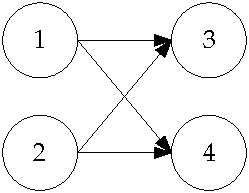
\includegraphics[width=1.3in,height=1in]{./image5} &

\includegraphics[width=1.2in,height=1in]{./image6} & 
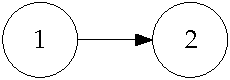
\includegraphics[width=1.2in,height=0.41in]{./image7} \\
a & b & c \\
\end{tabular}

\caption{Activity on Node (AON) representations of
activities. (a) Activity 1 must be completed before activity 2 can
begin. (b) Activities 1 and 2 must be completed before activity 3 can
begin. (c) Activity 1 and 2 must be completed before activities 3 and 4
can begin.}
\label{figure:activityOnNode}
\end{figure}


An example network diagram for a simple project is shown in 
Figure~\ref{figure:exampleNetworkDiagram}.
Dummy activity nodes for the start and end of the project have been
included. The ID number and estimated duration in days are indicated
inside each node. A given network diagram will have multiple paths from
the start to the end of the project. A path is any connected sequence of
activities from the start node to the end node. In this example, there
are four paths to completion:
$P_1 = \{1,4\} , P_2 = \{1,5\}, P_3 = \{2,3,4\}, P_4 = \{2,3,5\}$.
The completion of an individual path does not result in completion of
the project---all paths (and consequently all activities) must be
completed for the entire project to finish.

\begin{figure}[h]
\centering

\includegraphics[width=3.4in,height=0.96in]{./image12}
\caption{Example network diagram. Each activity contains the
activity ID and the estimated duration in days.}
\label{figure:exampleNetworkDiagram}
\end{figure}

The duration of each path is determined by summing the duration of all
activities on the path, which in this case is 20, 26, 28, and 34 days
for paths $P_1$ to $P_4$
respectively. The path with the longest duration is known as the
\emph{\textbf{critical path}} since it represents the minimum time
required to complete the project. In this example the critical path is
$P_4$.
Activities on the critical path are of particular interest, since, if
they fall behind schedule, or experience \emph{\textbf{slippage}}, the
overall completion time of the project is delayed. The other paths can
become critical paths if their activities experience sufficient slippage
to form a new critical path. A quantity known as \emph{\textbf{float}}
quantifies this margin. Float is the amount of time an activity can slip
without extending the overall completion time of the project. Thus, all
activities on the critical path have zero float by definition. The
following method is utilized to determine the float for activities:

\begin{enumerate}
\def\labelenumi{\arabic{enumi}.}
\item
  Identify all paths on the network diagram and the duration for each
  path.
\item
  The path with the longest duration is the critical path. Label the
  critical path duration as $t_{cp}$
  All activities on the critical path have zero float.
\item
  To determine the float for an activity that is not on the critical
  path, find all paths that the activity lies on and identify the one
  with the longest duration. Label this as $t_{lp}$ The float for the
  activity is calculated as
\end{enumerate}


\begin{equation}
\label{equ:floatTime}
Float = t_{cp} - t_{lp}
\end{equation}



Examples~\ref{example:projectManagementFloatTime} and 
\ref{example:projectManagementNetworkDiagram} examine float time computation.

\begin{example}{ Float time calculation.}
\label{example:projectManagementFloatTime}
\emph{\textbf{\ul{Problem:}}} Calculate the float for activities in the
network diagram shown in Figure~\ref{figure:exampleNetworkDiagram}.

\emph{\textbf{\ul{Solution:}}} The first two steps of the process have
already been completed, which are the identification of the paths, their
duration, and the critical path. To summarize, the paths are
$P_1 = \{1,4\}, P_2=\{1,5\}, P_3 =\{2,3,4\}, \text{ and } P_4 =\{2,3,5\}$
with durations of 20, 26, 28, and 34 days. The critical path is$P_4$
and $t_{cp}=34$ days, so activities 2, 3, and 5 have zero float. Thus

$$Float_{2,3,5} = 0 \text{ days}$$

The only two activities that are not on the critical path are 1 and 4.
Let's examine activity 1 first. It lies on paths $P_1$ and $P_2$
durations 20 and 26 days, thus the longest path to completion
$t_{lp1}$, for activity 1 is 26 days. The float is calculated from 
equation~\ref{equ:floatTime} as 
$Float_{1} =t_{cp} - t_{lp1} = 34-26 \text{days} = 8 \text{ days}$.

Activity 4 lies on $P_1$ and $P_3$, so $t_{lp4} = 28$ days and the float is

$$Float_{4} = t_{cp} - t_{lp4} = 34 -28 \text{ days} = 6 \text{ days}$$

This means that activity 1 can slip by 8 days and activity 4 can slip by
6 days without impacting the time to complete the project.
\end{example}

\begin{example}{Network diagram construction and float time
calculation for the temperature display.}
\label{example:projectManagementNetworkDiagram}

\emph{\textbf{\ul{Problem:}}} For the example WBS in 
Table~\ref{table:workBreakDownStructureExample}, (a)
create a network diagram, (b) determine the critical path and project
completion time, and (c) determine the float for all activities not on
the critical path.\\

\textbf{\ul{\emph{Solution:}}}
(a) The network diagram is constructed from the dependencies identified
in Table~\ref{table:workBreakDownStructureExample} and is shown below.


\includegraphics[width=4.2in,height=1.74in]{./image22} \\

(b) The three paths from start to end are: $P_1 = \{1.1, 1.2, 1.3.1, 1.3.3, 3\}$, \\
$P_2 = \{1.1, 1.2, 1.3.2, 1.3.3, 3\}$, and $P_3 = \{2.1, 2.2, 2.3, 2.4, 3\}$
which have durations of 38, 39, and 30 days respectively. Thus the
\ul{critical path} is $P_2$ and its duration is

$$t_{cp} = 39 \text{ days}$$ \\

(c) All activities on path $P_1$ are also part of
the critical path, with the exception of activity 1.3.2, which has

$$Float_{1.3.2} = 39 - 38 \text{ days} = 1 \text{ day}$$

Activities 2.1-2.4 have the collective float

$$Float_{2.1-2.4} = 39 - 30 \text{ days} = 9 \text{ days}$$
\end{example}

The strength of the network diagram is that it provides an intuitive
graphical representation of activities and their dependencies on one
another. This is particularly valuable for complex projects where the
paths to completion may not be obvious. It also allows identification of
the critical path and float times for activities. A disadvantage of the
network diagram is that it may be difficult to encapsulate the amount of
information required for an in-depth project on a single page in an easy
to read format.

\section{Gantt Charts}
\label{section:gantt-charts}

\emph{\textbf{Gantt charts}}, developed by a mechanical engineer named
Henry Gantt (1861-1919), are a bar graph representation of activities on
a timeline. An example Gantt chart is shown in Figure~\ref{figure:ghantChart} for the
temperature display design. The Gantt chart effectively shows the WBS
and the timeline for completion. A traditional weakness of the Gantt
chart has been the inability to show the dependencies between
activities. However, as seen in this example, this has been remedied by
modern project management software where the dependencies are indicated
by the connecting arrows between tasks.

\begin{figure}[h]
\centering

\includegraphics[width=5.5in,height=3.8in]{./image28}
\caption{Gantt chart for the temperature display project
created using Microsoft Visio\textsuperscript{TM}}
\label{figure:ghantChart}
\end{figure}


\section{Cost Estimation}
\label{section:cost-estimation}

The second main objective of this chapter is to address how to complete
projects within budget. In order to do this, the costs associated with
the design, development, and manufacture of the system need to be
estimated. This section describes break-even cost analysis and economic
considerations followed by methods of cost estimation.

\subsection{Break-Even Analysis}
\label{subsection:break-even-analysis}

A break-even analysis aims to determine the number of units that must be
sold for costs and revenues to be equal---in other words, for there to
be no profit or loss. The two types of costs that factor into this
analysis are fixed and variable costs. \emph{\textbf{Fixed costs}} are
those that are constant regardless of the number of units produced and
cannot be directly charged to a process or activity. Examples are rent,
overhead, insurance, property taxes, design and development costs,
capital expenditures, market research, and sometimes labor costs
depending upon the situation. Capital expenditures are costs incurred
for long-term assets such as equipment or buildings.
\emph{\textbf{Variable costs}} vary depending upon the process or items
being produced, and fluctuate directly with the number of units
produced. Examples are raw materials, inventory, energy costs, and labor
costs.

The \emph{\textbf{break-even point}} is the point where the number of
units sold is such that there is no profit or loss. It is determined
from the total costs and revenue. The total cost required to produce a
product is the sum of fixed and variable costs. Assuming \emph{n} units
are sold, the total cost is

\begin{equation}
\label{equ:totalCost}
\text{Total cost} = \text{fixed cost} + n *\frac{\text{variable cost}}{\text{unit}}
\end{equation}

The total revenue generated by the sale of the \emph{n} units is
directly related to the sale price

\begin{equation}
\label{equ:Revenue}
\text{Reveneue} = n *\frac{\text{sales price}}{\text{unit}}
\end{equation}

The break-even point is where the revenue and total costs are equal

\begin{equation}
\label{equ:breakEven}
n * \frac{\text{sales price cost}}{\text{unit}} = \text{fixed cost} + n * \frac{\text{variable cost}}{\text{unit}}
\end{equation}

The break-even analysis is shown graphically in 
Figure~\ref{figure:breakEvenGraph} with the
costs and revenue plotted as a function of units sold. 
Equation~\ref{equ:breakEven}
allows different scenarios to be examined. For example, based upon a
certain cost structure and sales price, the volume of sales necessary to
break-even can be computed. Or, based upon a cost structure and
projected number of units sold, a target sales price can be selected.
Example~\ref{example:projectManagementBreakEvenHpPrinter} 
demonstrates the application of break-even analysis for the
development of the Hewlett-Packard (HP) DeskJet printer.

\begin{figure}[h]
\centering

\includegraphics[width=4.8in,height=3.36in]{./image32}
\caption{Graphical representation of the break-even
analysis.}
\label{figure:breakEvenGraph}
\end{figure}



\begin{example}{ Break-even analysis for the HP DeskJet printer.}
\label{example:projectManagementBreakEvenHpPrinter}

\emph{\textbf{\ul{Problem:}}} The following data has been publicly
reported for the development and sale of the HP DeskJet {[}Ulr03{]}:
sales price = \$300, development cost = \$50 million, production
investment = \$25 million, annual production (sales) volume = 4 million
units per year, and the sales lifetime is 2 years. Assuming a fictitious
variable production cost of \$225/unit, determine: (a) the number of
units that must be sold to break even, and (b) the profit expected over
an estimated sales lifetime of 2 years.\\

\emph{\textbf{\ul{Solution:}}}

(a) The objective is to determine the sales volume, \emph{n,} necessary
to break even. The fixed costs are the sum of the development costs and
production investment. So

$$\text{Fixed costs} = \$(50+25) \text{million} = \$75 \text{ million}$$
This leads to a total cost for \emph{n} units sold of
$$\text{Total cost} = \$75 \text{million} + n x \$225$$
The revenue is
$$\text{Revenue} = n * 300$$
Setting the revenue and total cost each equal at the break-even point
produces
$$n * \$400 = \$75 \text{ million} + n * \$225$$
Solving for the final number of units gives
$$N = 1 \text{ million}$$\\

(b) Profit is the differential between the total revenue and the total
cost and is expressed as
$$ \text{Profit = total revenue - total costs}$$
For an expected volume of 4 million units per year over 2 years
$$\text{Profit} = n * \$300 - (\$ 75 \text{ million} + n * \$225)$$
$$   = 8 \text{ million} * \$300 - (\$ 75 \text{ million} + 8 \text{ million} * \$225)$$
$$\text{Profit} = \$525 \text{ million}$$
\end{example}

\subsection{Cost Models}
\label{subsection:cost-models}

The costs must be accurately estimated in order to realize the expected
profit. The goal here is not to address the complete subject of cost
estimation, which is beyond the scope of this book, but instead present
some basic concepts and techniques for estimating development costs.
Many projects go over budget during development, and this is a
particularly important consideration from a design viewpoint. The WBS is
a valuable tool for cost estimation because it divides the project into
manageable pieces whose individual costs can be more readily estimated.

As identified in the WBS, the development costs associated with a
project typically include labor, equipment, and materials. Equipment
costs can be determined in a fairly straightforward manner, because many
of the equipment needs are known \emph{a priori}. Labor costs are tied
directly to the length of the project and are often the largest expense.

Estimates of labor costs are usually based upon past experience and
expert opinion. This means asking others to estimate the cost and use it
as a guide. The estimation formula in (1) for activity duration can be
applied for costs as

\begin{equation}
\label{equ:costEstimateFormula}
Cost \frac{cost_a +4 cost_m + cost_b}{6}
\end{equation}

where $cost_a$ is the most optimistic
cost estimate, $cost_m$ is the most
likely cost estimate, and $cost_b$ is the
most pessimistic cost estimate.

A more formal approach for estimating labor costs is to use empirical
models that represent a quantification of past experience. The models
estimate an output based upon quantifiable inputs related to the design
or technology. Example inputs are the number of subsystems, the
estimated complexity of a circuit design, or an estimate of the lines of
code necessary for a software project. This changes the problem from
opinion-based estimation to estimation of a quantity that is presumably
easier to find and a better indicator of the cost. The output of the
model is the cost or another quantity that is directly related to it,
such as the estimated number of person-hours.

The simplest example is a linear model $y=mx+b$ for estimating an
output $y$ (cost or person-hours) based upon an input $x$. For
example, IBM modeled software development project costs using the number
of lines of code as the input {[}Jal97{]} as

\begin{equation}
\label{equ:softwareEffortIBM}
\text{Effort} = a * KLOC + b
\end{equation}

The output is an estimate of the effort in person-months and the input
is the projected number of lines of code, KLOC. KLOC, pronounced
``kayloc'', equals thousands (kilo) of lines of code. The linear model
was found to work well for relatively small development projects with
between 4 and 10 KLOC. As the complexity increased, an exponential model
was found to be more realistic where

\begin{equation}
\label{equ:softwareEffortExp}
\text{Effort} = a(KLOC)^b
\end{equation}

By observation of 60 software development projects at IBM, the
exponential model was fit to observed data and the parameters were
estimated to be $a=5.2$ and $b = 0.91$. The KLOC model is
applied in Example~\ref{example:projectManagementEffortEstimation}.

\begin{example}{Effort estimation using KLOC.}
\label{example:projectManagementEffortEstimation}

\emph{\textbf{\ul{Problem:}}} Consider a software development project
that has a team of 10 software development engineers. The team has
proposed a design and estimates that it will require 50,000 lines of
code to complete the project. The average cost to the company for an
engineer is \$100,000 per year, including salary, benefits, and
overhead. Estimate (a) the time required to the complete the project and
(b) the labor costs. \\

\emph{\textbf{\ul{Solution:}}}

(a) Based upon the projected value KLOC, the exponential model in
equation~\ref{equ:softwareEffortExp} is
most appropriate

$$\text{Effort} = 5.2(50)^{0.91} = 183 \text{ worker months}$$

Since there are 10 developers on the project, the estimated time is
determined by dividing the effort by 10, to produce an estimated time of
\ul{18.3 months}.\\

(b) The labor costs for development are determined from the number of
person-months and the average monthly salary of a development engineer
as

$$\text{Labor cost} = \text{183 worker-months}  * \frac{\$100,000}{\text{year}} * \frac{\text{1 year}}{\text{12 months}}$$
$$\text{Labor cost} = \$1.53 \text{ million}$$
\end{example}

The models in 
equations~\ref{equ:softwareEffortIBM} and \ref{equ:softwareEffortExp}
 are simplistic in that there is a single input
to the estimator. For example, what if there were 100 engineers assigned
to the project in Example~\ref{example:projectManagementEffortEstimation}? 
The model indicates that the project
would be completed in 1.83 months at the same cost. Common sense
dictates that this is unrealistic; this problem is commonly referred to
as the ``mythical man-month'' (person-month). The mythical person-month
refers to the fact that just adding more people to the team will not
linearly reduce development time. The reality is that many factors
impact the costs, which leads to effort estimation based on many inputs.
An example of this is the Constructive Cost Model (COCOMO) that is also
used in software development. There are different levels of COCOMO that
allow increasingly complex model inputs, such as the type of technology
employed, the maturity of the technology, the size of the team, the
experience of the engineers, and the timeframe required to complete the
project. Not only do the models estimate costs, but they can also be
used to estimate how many engineers are needed to complete projects of a
given complexity. Although the examples cited here are from the software
field, the concepts are general and applicable to the development of
many technologies.

Empirical cost models can also be developed for the materials necessary
for the manufacture of items. Material estimates are often based upon
the expected size and types of technologies used in the manufactured
part. For example, a cost model for the manufacture of a printed circuit
board may have as inputs the size of the board, the number of layers,
and the type of technology used (such as through-hole vs. surface
mount).

\section{The Project Manager}
\label{section:the-project-manager}

Many engineering teams have a project manager responsible for planning
and organizing the project. The project manager may take primary
responsibility for developing the WBS, the network diagram and Gantt
chart, the cost estimates, and the budget. Although the project manager
may have primary responsibility for the project plan, all team members
should have input and contribute to development of the plan. The project
manager should monitor the checkpoints and deliverables against the plan
and develop strategies for reacting to slippage in any activities. The
plan should be updated as necessary and the changes communicated to all
involved. The project manager may also have primary responsibility for
the purchasing of materials and controlling spending. Project managers
are not necessarily the boss in the traditional sense and should be
viewed as member of the team. As such, it is important for the project
manager to also be responsible for completing project deliverables in
addition to the project management tasks.

\section{Guidance}
\label{section:projectManagementGuidance}

The following is guidance to consider when creating the project
management plan, and is particularly relevant for those working on
capstone design projects:

\begin{itemize}
\item
  \emph{Build the plan after the design architecture is complete.} The
  project plan can be created at any point in the design process. Our
  experience shows that a good time to develop it is after the system
  design architecture is complete. The design serves as a good guide for
  developing the WBS.
\item
  \emph{Take the initial time estimates for activities and double them!}
  Most people tend to significantly underestimate the amount of time it
  takes to complete an activity. That is because people often have a
  conceptual idea of what it will take to complete the task and can
  envision the steps to completion. The desire to please superiors also
  influences people to underestimate the time to completion. Although it
  may not be necessary to double the time estimates, you can incorporate
  the most optimistic and pessimistic estimates and apply 
Equation~\ref{equ:projectTimeEstimate}
  Or, if a proven mathematical model exists, such as the KLOC estimator
  in Equations~\ref{equ:softwareEffortIBM} and \ref{equ:softwareEffortExp}, 
it can be used to estimate times.
\item
  \emph{Assign a lot of time for testing and integration.} During
  integration many people must work together to integrate components
  that may have been developed in isolation. Problems with a single
  component can bring the integration to a halt. Delays may be
  compounded by necessary re-design to correct the problem.
\item
  \emph{Factor in lead times for part ordering.} Even with the Internet
  and overnight delivery, you may find that needed parts and equipment
  are out-of-stock. Lead times for seemingly commonplace items can
  sometimes be quite lengthy.
\item
  \emph{Assign a project manager(s).} Consider assigning one individual
  who has primary responsibility for organizing and monitoring the plan.
  Again, the project manager must also be responsible for some of the
  deliverables for completion of the project.
\item
  \emph{Do not assign all team members to all tasks.} Experience shows
  that when this is the case nobody is responsible for anything and the
  work doesn't get done. There needs to be individual accountability for
  all team members. However, it may be a good idea to have more than one
  person responsible for activities for backup support as shown in the
  WBS in Table~\ref{table:workBreakDownStructureExample}.
\item
  \emph{Track the progress versus the plan.} There is a tendency to
  create the plan and then ignore it. The plan is only valuable if it is
  monitored and progress is tracked.
\item
  \emph{Don't become a slave to the plan.} Circumstances usually dictate
  change. Be prepared to shift resources as needed. Monitor the plan to
  see if there are changes to the critical path or if a new critical
  path emerges.
\item
  \emph{Experience counts.} Get started now in developing this
  experience by creating a plan for your project.
\end{itemize}

\section{Project Application: The Project Plan}
\label{section:project-application-the-project-plan}

A project plan should contain the following:

\begin{itemize}
\item
  \emph{Work Breakdown Structure}. Identify the activities,
  deliverables, responsibilities, duration, resources, and dependencies
  as demonstrated in 

Table~\ref{table:workBreakDownStructureExample}. Be sure to 
provide sufficient detail in
  the structure and identify clear deliverables.
\item
  \emph{Gantt Chart and/or Network Diagram.} Provide a graphical
  representation of the project plan. Network diagrams have the
  advantage of showing the dependencies, while Gantt charts show the
  timeframe. Modern software tools allow both to be integrated into the
  same graph and are a good compromise as demonstrated in 
Figure~\ref{figure:ghantChart}.
  The critical path should be identified and the float for non-critical
  path activities understood.
\item
  \emph{Costs.} Develop a tabulated list of costs and for the equipment,
  materials, and labor necessary to carry out the project. It may not be
  necessary to develop labor costs for a capstone project, yet it is
  good practice to estimate person-hours and compare the estimate to the
  actual at the end of the project.
\end{itemize}

\section{Summary and Further Reading}
\label{section:projectManagementSummary-and-further-reading}

Three main objectives of project management are to complete projects
that are on-time, within budget, and meet the needs of the user. This
chapter addressed the time and budget aspects. The key element in
developing a project plan is the WBS, which is a hierarchical
identification of the activities needed to complete the project. Both
network diagrams and Gantt charts can be created from the WBS. A network
diagram is a graphical representation of activities and their
dependencies that provides for quantitative analysis of the project
plan. This analysis includes computation of the critical path and float
times. The Gantt chart is related to the network diagram, but provides a
time scale representation of the activities. In terms of the budget
issues, a simple profit and loss model was presented with a break-even
analysis. Model-based techniques can be used for estimating labor costs,
where the models are built from the analysis of similar projects. The
models can be linear or nonlinear with single inputs. More complex
models can be developed with multiple inputs in order to arrive at a
more precise estimate.

Project management is a well developed field and there are many good
textbooks and online resources available for delving deeper into the
subject. \ul{Project Management} by Gray and Larson {[}Gra02{]} is a
comprehensive text on the subject that includes risk management,
resource scheduling, leadership, and performance measurement.\\
\ul{Planning, Performing, and Controlling Projects} by Angus et al.
{[}Ang00{]} is written for an engineering and scientific audience, and
integrates phases of the design process. MindTools
(\href{http://www.mindtools.com}{www.mindtools.com}) is an online
resource that addresses many career skills including project management.
